%!TEX root = ../main.tex

\chapter{Antenna}

\section{Struttura generale}
Nella parabola (versione 1.0 revisione 2) del kit fornito da Starlink troviamo sul retro dell'antenna una coppia di motori e un cavo ethernet che si collega al router.
Questi motori non muovono continuamente la parabola per puntare direttamente al satellite con cui comunica; vengono utilizzati solo durante la configurazione iniziale per orientare l'antenna nella direzione generale corretta.
Nel retro dell'antenna troviamo una piastra posteriore strutturale in alluminio e, dall'altro lato, una grande scheda a circuiti stampati (PCB).
Su un lato ci sono 640 microchip piccoli e 20 microchip più grandi, disposti in un pattern con tracce che si diramano dai microchip più grandi a quelli più piccoli, insieme a chp aggiuntivi, inclusa la CPU principale e il modulo GPS sul bordo del PCB. Sull'altro lato cisono circa 1400 cerchi di rame con una griglia di quadrati tra i cerchi.
Nel livello successivo c'è uno schema a nido d'ape in gomma con piccoli cerchi di rame intagliati e dietro troviamo un altro schema a nido d'ape e poi la copertura anteriore della parabola.
Abbiamo quindi 1280 antenne disposte in un pattern esagonale a nido d'ape, con ciascuna pila di cerchi di rame che rappresenta una singola antenna controllata dai microchip sul PCB.
Questo enorme array funziona insieme in quella che è chiamata un'antenna phased array per inviare e ricevere onde elettromagnetiche che vengono direzionate verso e da un satellite Starlink in orbita a 550km di distanza \cite{branch_education_how_2022}.

\subsection{Funzionamento dell'antenna Aperture Coupled Patch}

\begin{figure}[htbp]
  \centering
  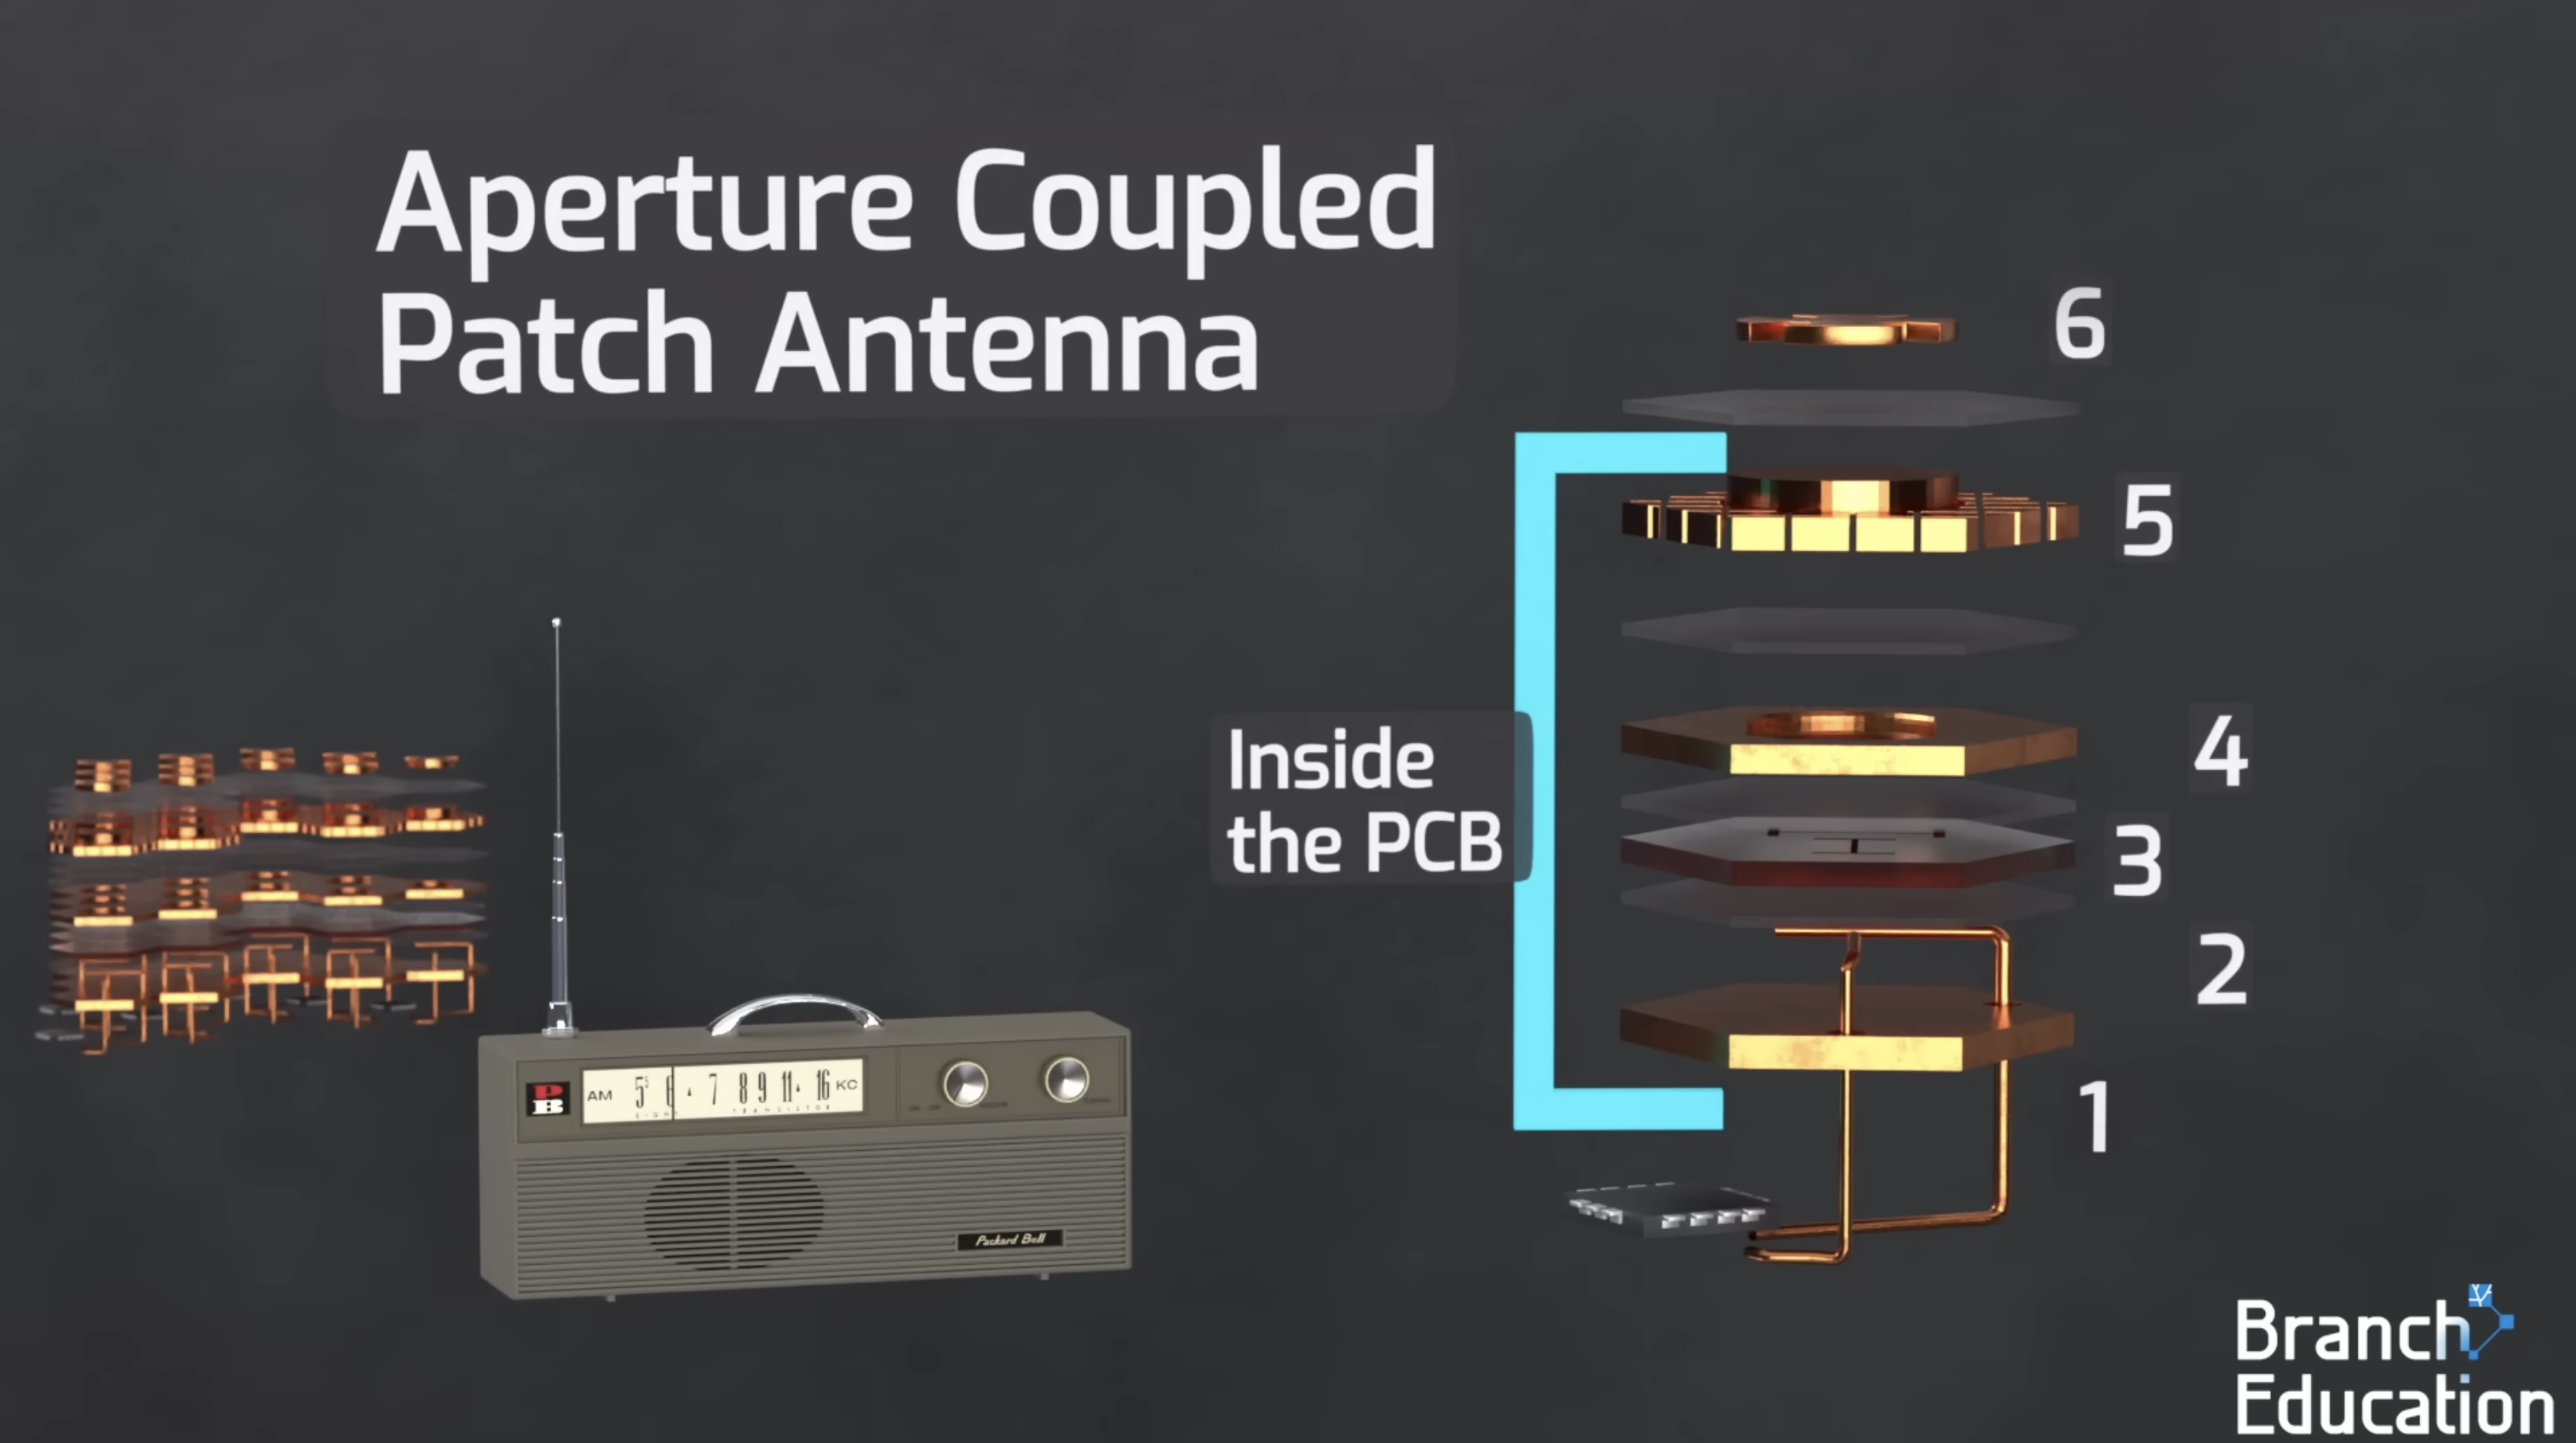
\includegraphics[width=0.8\linewidth]{./res/img/antenna_pcb.png}
  \caption{Aperture Coupled Patch antenna \cite{branch_education_how_2022}.}
  \label{fig:aperture-couple-patch-antenna}
\end{figure}

Nella figura \ref{fig:aperture-couple-patch-antenna} possiamo vedere un'aperture coupled patch antenna, composta di 6 layer, il più dei quali all'interno del PCB.
I layer più importanti sono:
\begin{itemize}
  \item[1.] Linea di alimentazione.
  \item[2.] Patch radiante che riflette le radiofrequenze.
  \item[3.] H slot per la polarizzazione. Servono per accoppiare l'energia dalla linea di alimentazione al patch radiante.
  \item[4.] Isolamento dell'antenna.
  \item[5.] Bottom antenna patch: trasmettitore a 13 GHz.
  \item[6.] Top antenna patch: ricevitore a 11.7 GHz.
\end{itemize}
I pezzi esagonali grigio scuro invece sono isolamento elettrico tra i vari layer \cite{branch_education_how_2022}.

Per facilitare la comprensione del suo funzionamento semplifichiamola rimuovendo per il momento alcuni layer, e vediamo i principi base di come si genera un'onda elettromagnetica che si propaga da quest'antenna.

Per iniziare, sul fondo abbiamo una micro linea di trasmissione elettrica che arriva da uno dei piccoli microchip.
Questa linea di trasmissione è solo un filo di rame che termina sotto la pila dell'antenna.
Mandiamo una tensione sinusodiale alla frequenza di 12 GHz al filo di alimentazione, quindi con un periodo di 83 picosecondi.
Al di sopra del filo di rame di alimentazione abbiamo un cerchio di rame con intagli chiamato patch d'antenna.

Con la corrente continua o alternata a bassa frequenza, non succederebbe molto perchè il patch è isolato, ma con un segnale ad alta frequenza la potenza inviata al filo di alimentazione viene accoppiata o inviata al patch.
Questo fenomeno avviene perchè quando la tensione è al fondo della sua sinusoide, o al minimo, c'è una concentrazione di elettroni spinti verso l'estremità del filo di alimentazione, creando così una zona di carica negativa che corrisponde alla massima tensione negativa.
Questa concentrazione di elettroni sulla punta del filo respinge tutti gli elettroni, compresi quelli sulla parte superiore del patch, e di conseguenza questi elettroni vengono spinti verso l'altro lato del patch circolare.
In questo modo, un lato del patch diventa carico positivamente, mentre l'altro diventa carico negativamente, creando così campi elettrici tra il patch e il filo di alimentazione.

Tuttavia, quando invertiamo la tensione al filo di rame 41.5 picosecondi dopo, abbiamo una concentrazione di cariche positive, o una mancanza di elettroni all'estremità del filo, e quindi gli elettroni nel patch fluiscono verso l'altro lato. La tensione nel patch è invertita e quindi anche la direzione dei campi elettrici è invertita \cite{branch_education_how_2022}.

\begin{figure}[htbp]
  \centering
  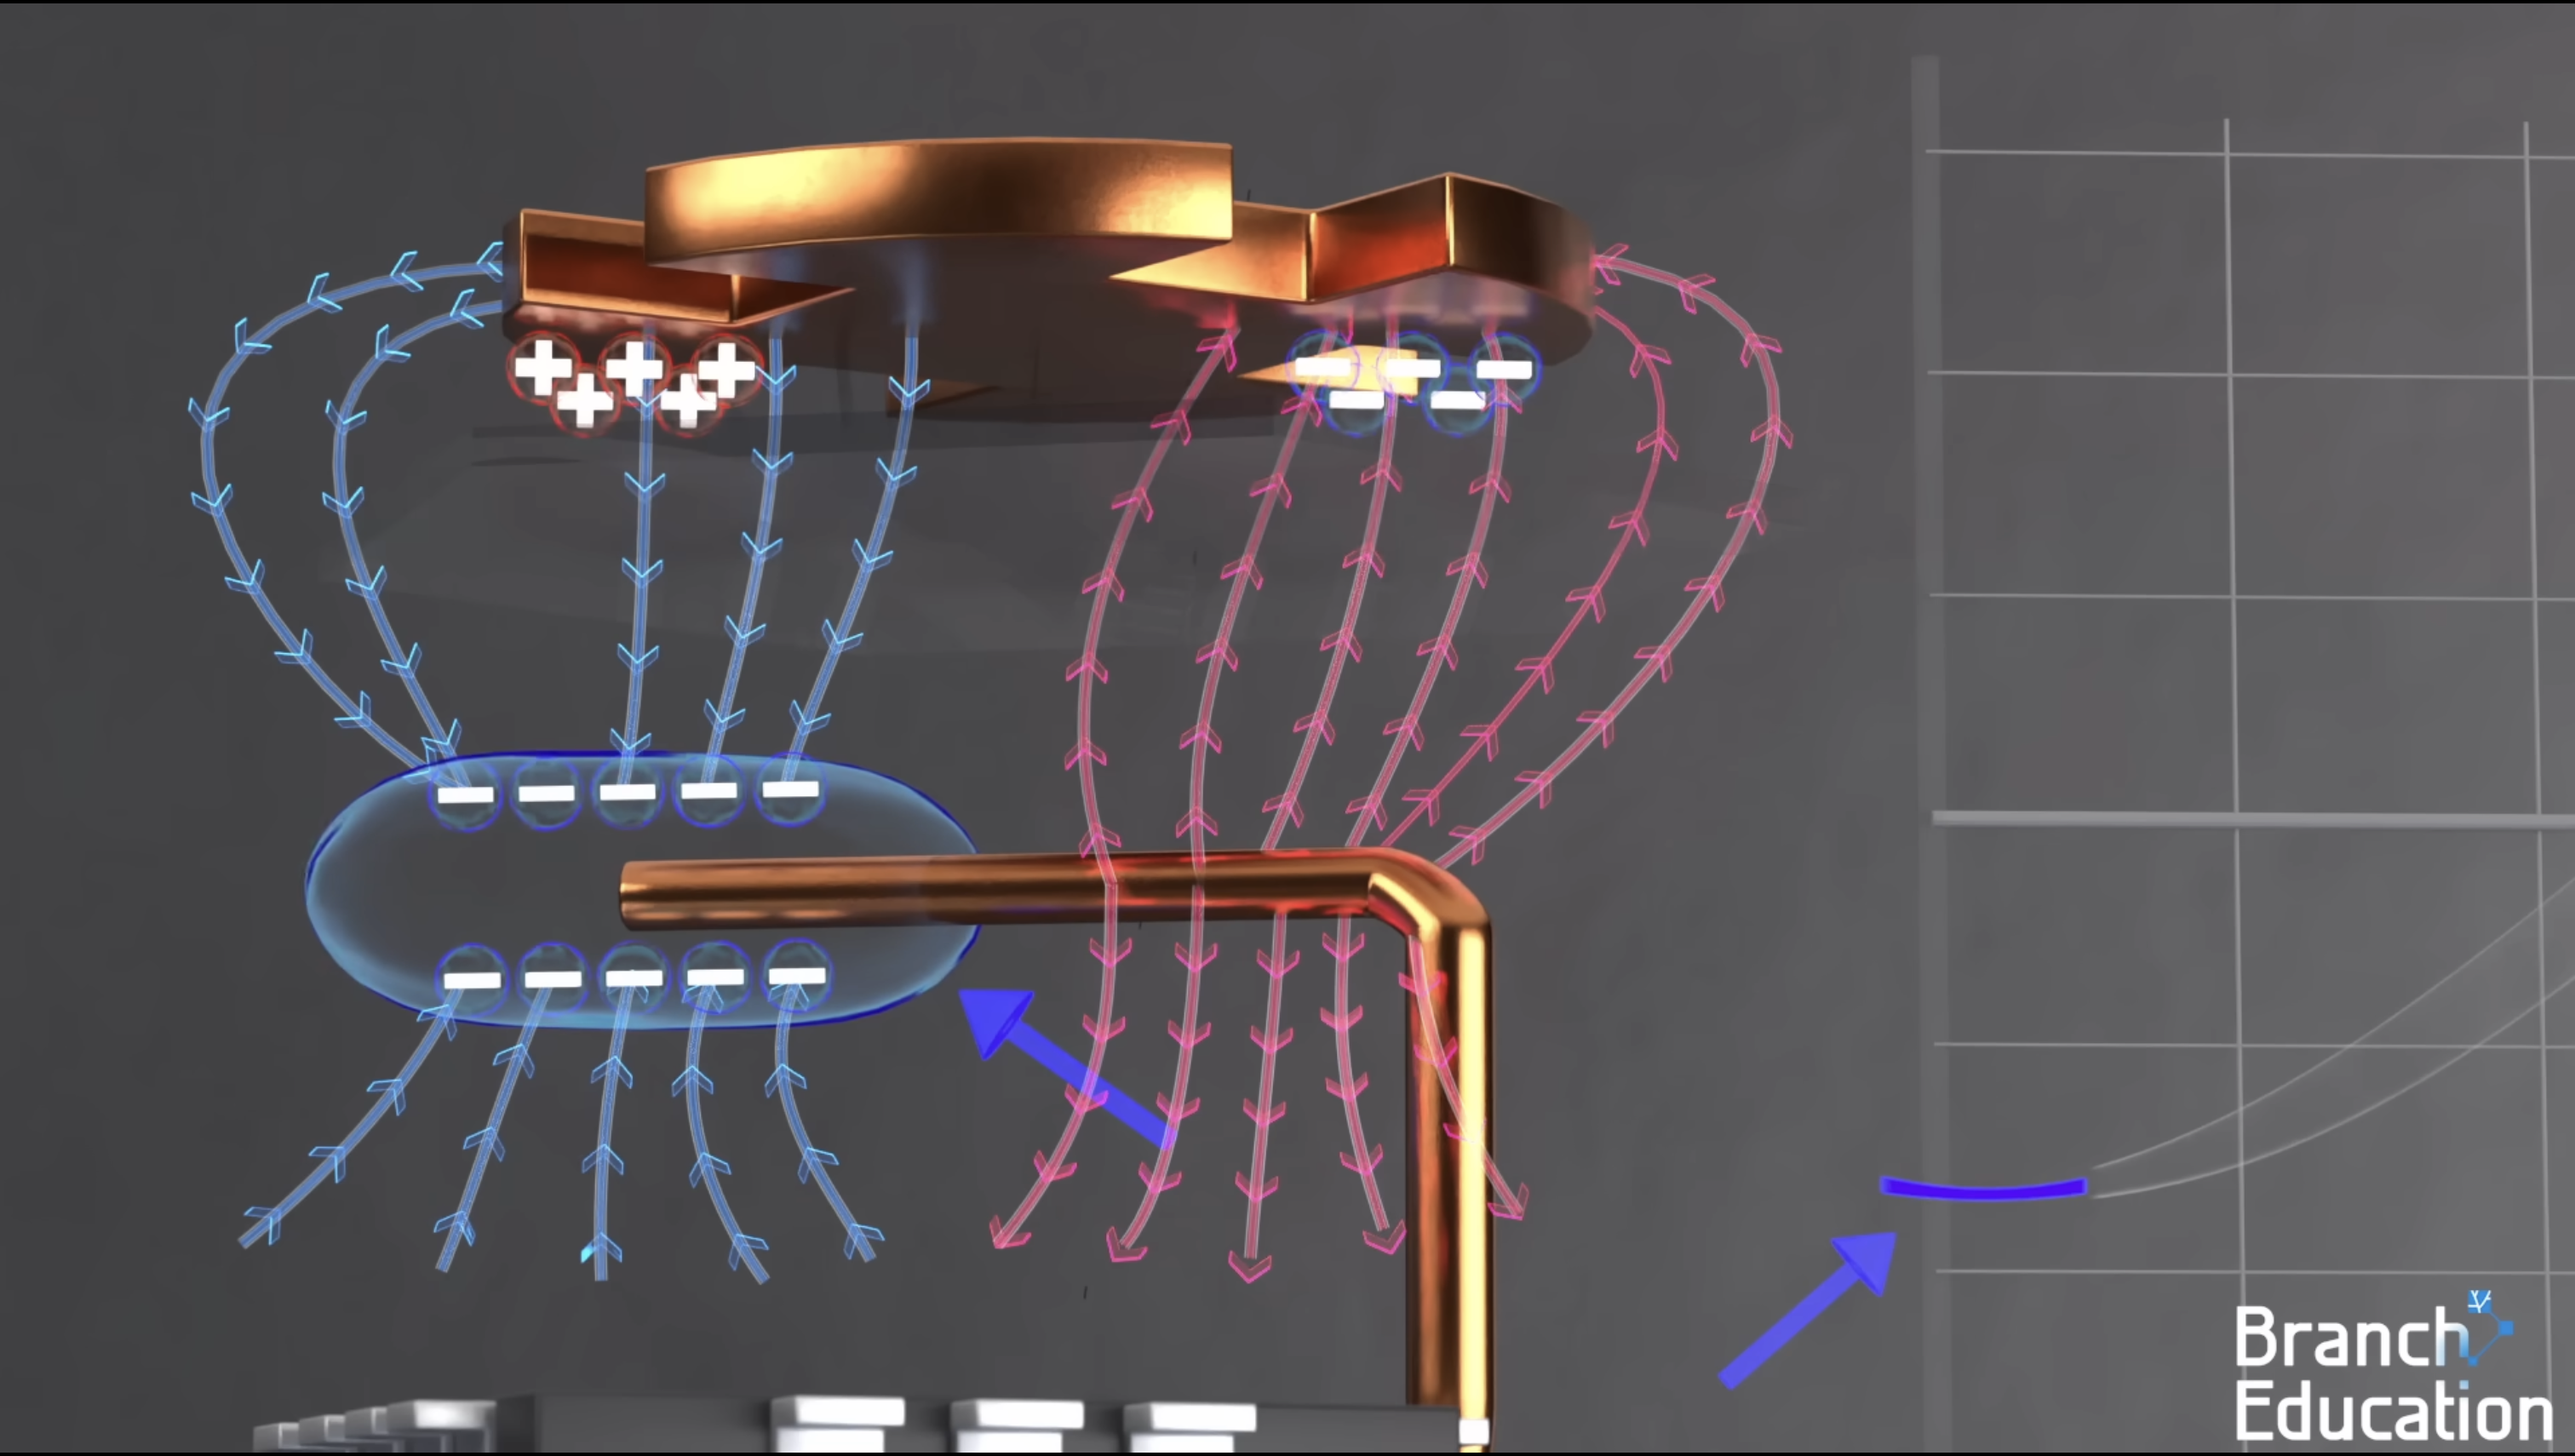
\includegraphics[width=0.8\linewidth]{./res/img/antenna_voltage_applied.png}
  \caption{Aperture Coupled Patch antenna con un segnale applicato \cite{branch_education_how_2022}.}
  \label{fig:aperture-couple-patch-antenna-voltage-applied}
\end{figure}

Poiché la tensione del filo di alimentazione oscilla con un intervallo di 41.5 picosecondi tra un picco e un avvallamento, anche i campi elettrici nel patch oscilleranno mentre gli elettroni vanno avanti e indietro.

\begin{figure}[htbp]
  \centering
  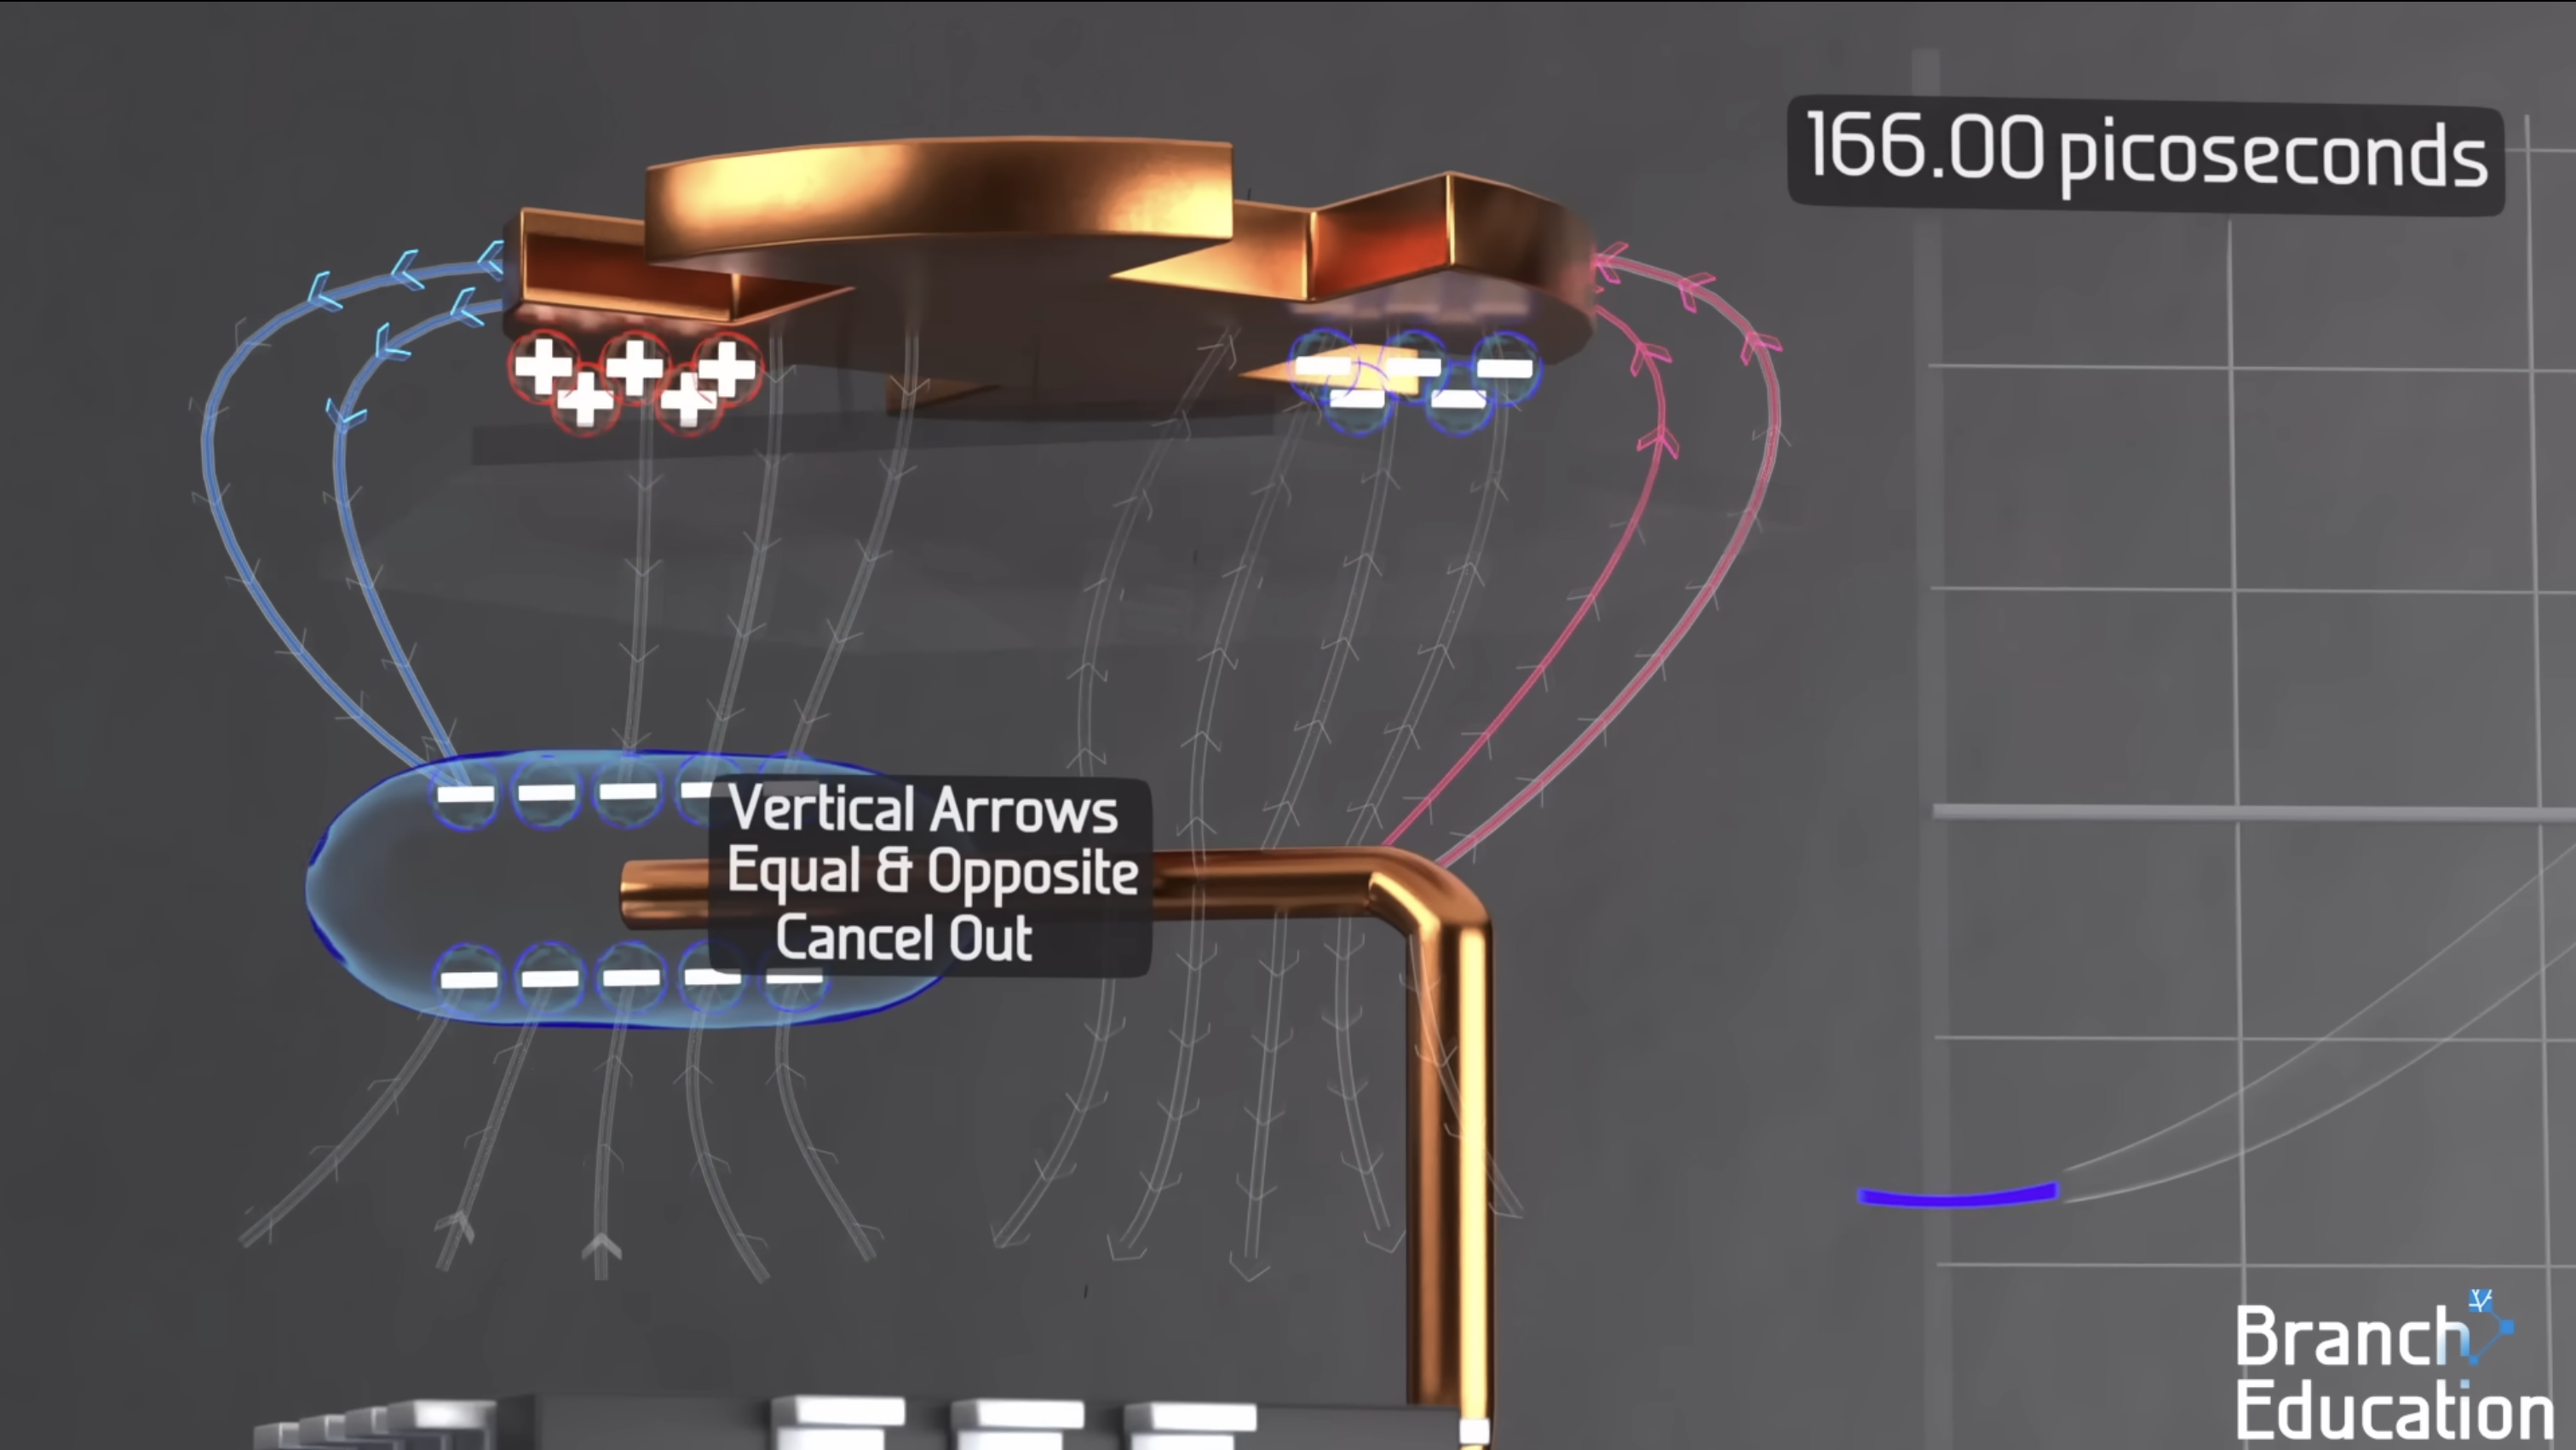
\includegraphics[width=0.8\linewidth]{./res/img/antenna_fringing_fields.png}
  \caption{Creazione dei campi di frangia in un'Aperture Coupled Patch antenna \cite{branch_education_how_2022}.}
  \label{fig:aperture-couple-patch-antenna-fringing-fields}
\end{figure}

Possiamo vedere in figura \ref{fig:aperture-couple-patch-antenna-fringing-fields} che alcuni di questi vettori di campo elettrico provenienti dal patch sono verticali e, poiché sono opposti, si annullano.
Tuttavia, altri campi elettrici sono orizzontali nello stesso piano del patch e sono chiamati campi di frangia.
Questi campi di frangia sono nella stessa direzione e quindi si sommano l'uno all'altro, dando luogo a un campo elettrico combinato \cite{branch_education_how_2022}.

Allo stesso tempo, gli elettroni che scorrono da un lato all'altro del disco, che costituiscono una corrente elettrica, generano un campo magnetico con un'intensità e una direzione, o vettore, perpendicolare al vettore del campo elettrico di frangia.
Di conseguenza, abbiamo un campo elettrico orientato in un senso e un campo magnetico orientato perpendicolarmente, come si può vedere in figura \ref{fig:aperture-couple-patch-antenna-em-field} \cite{branch_education_how_2022}.

\begin{figure}[htbp]
  \centering
  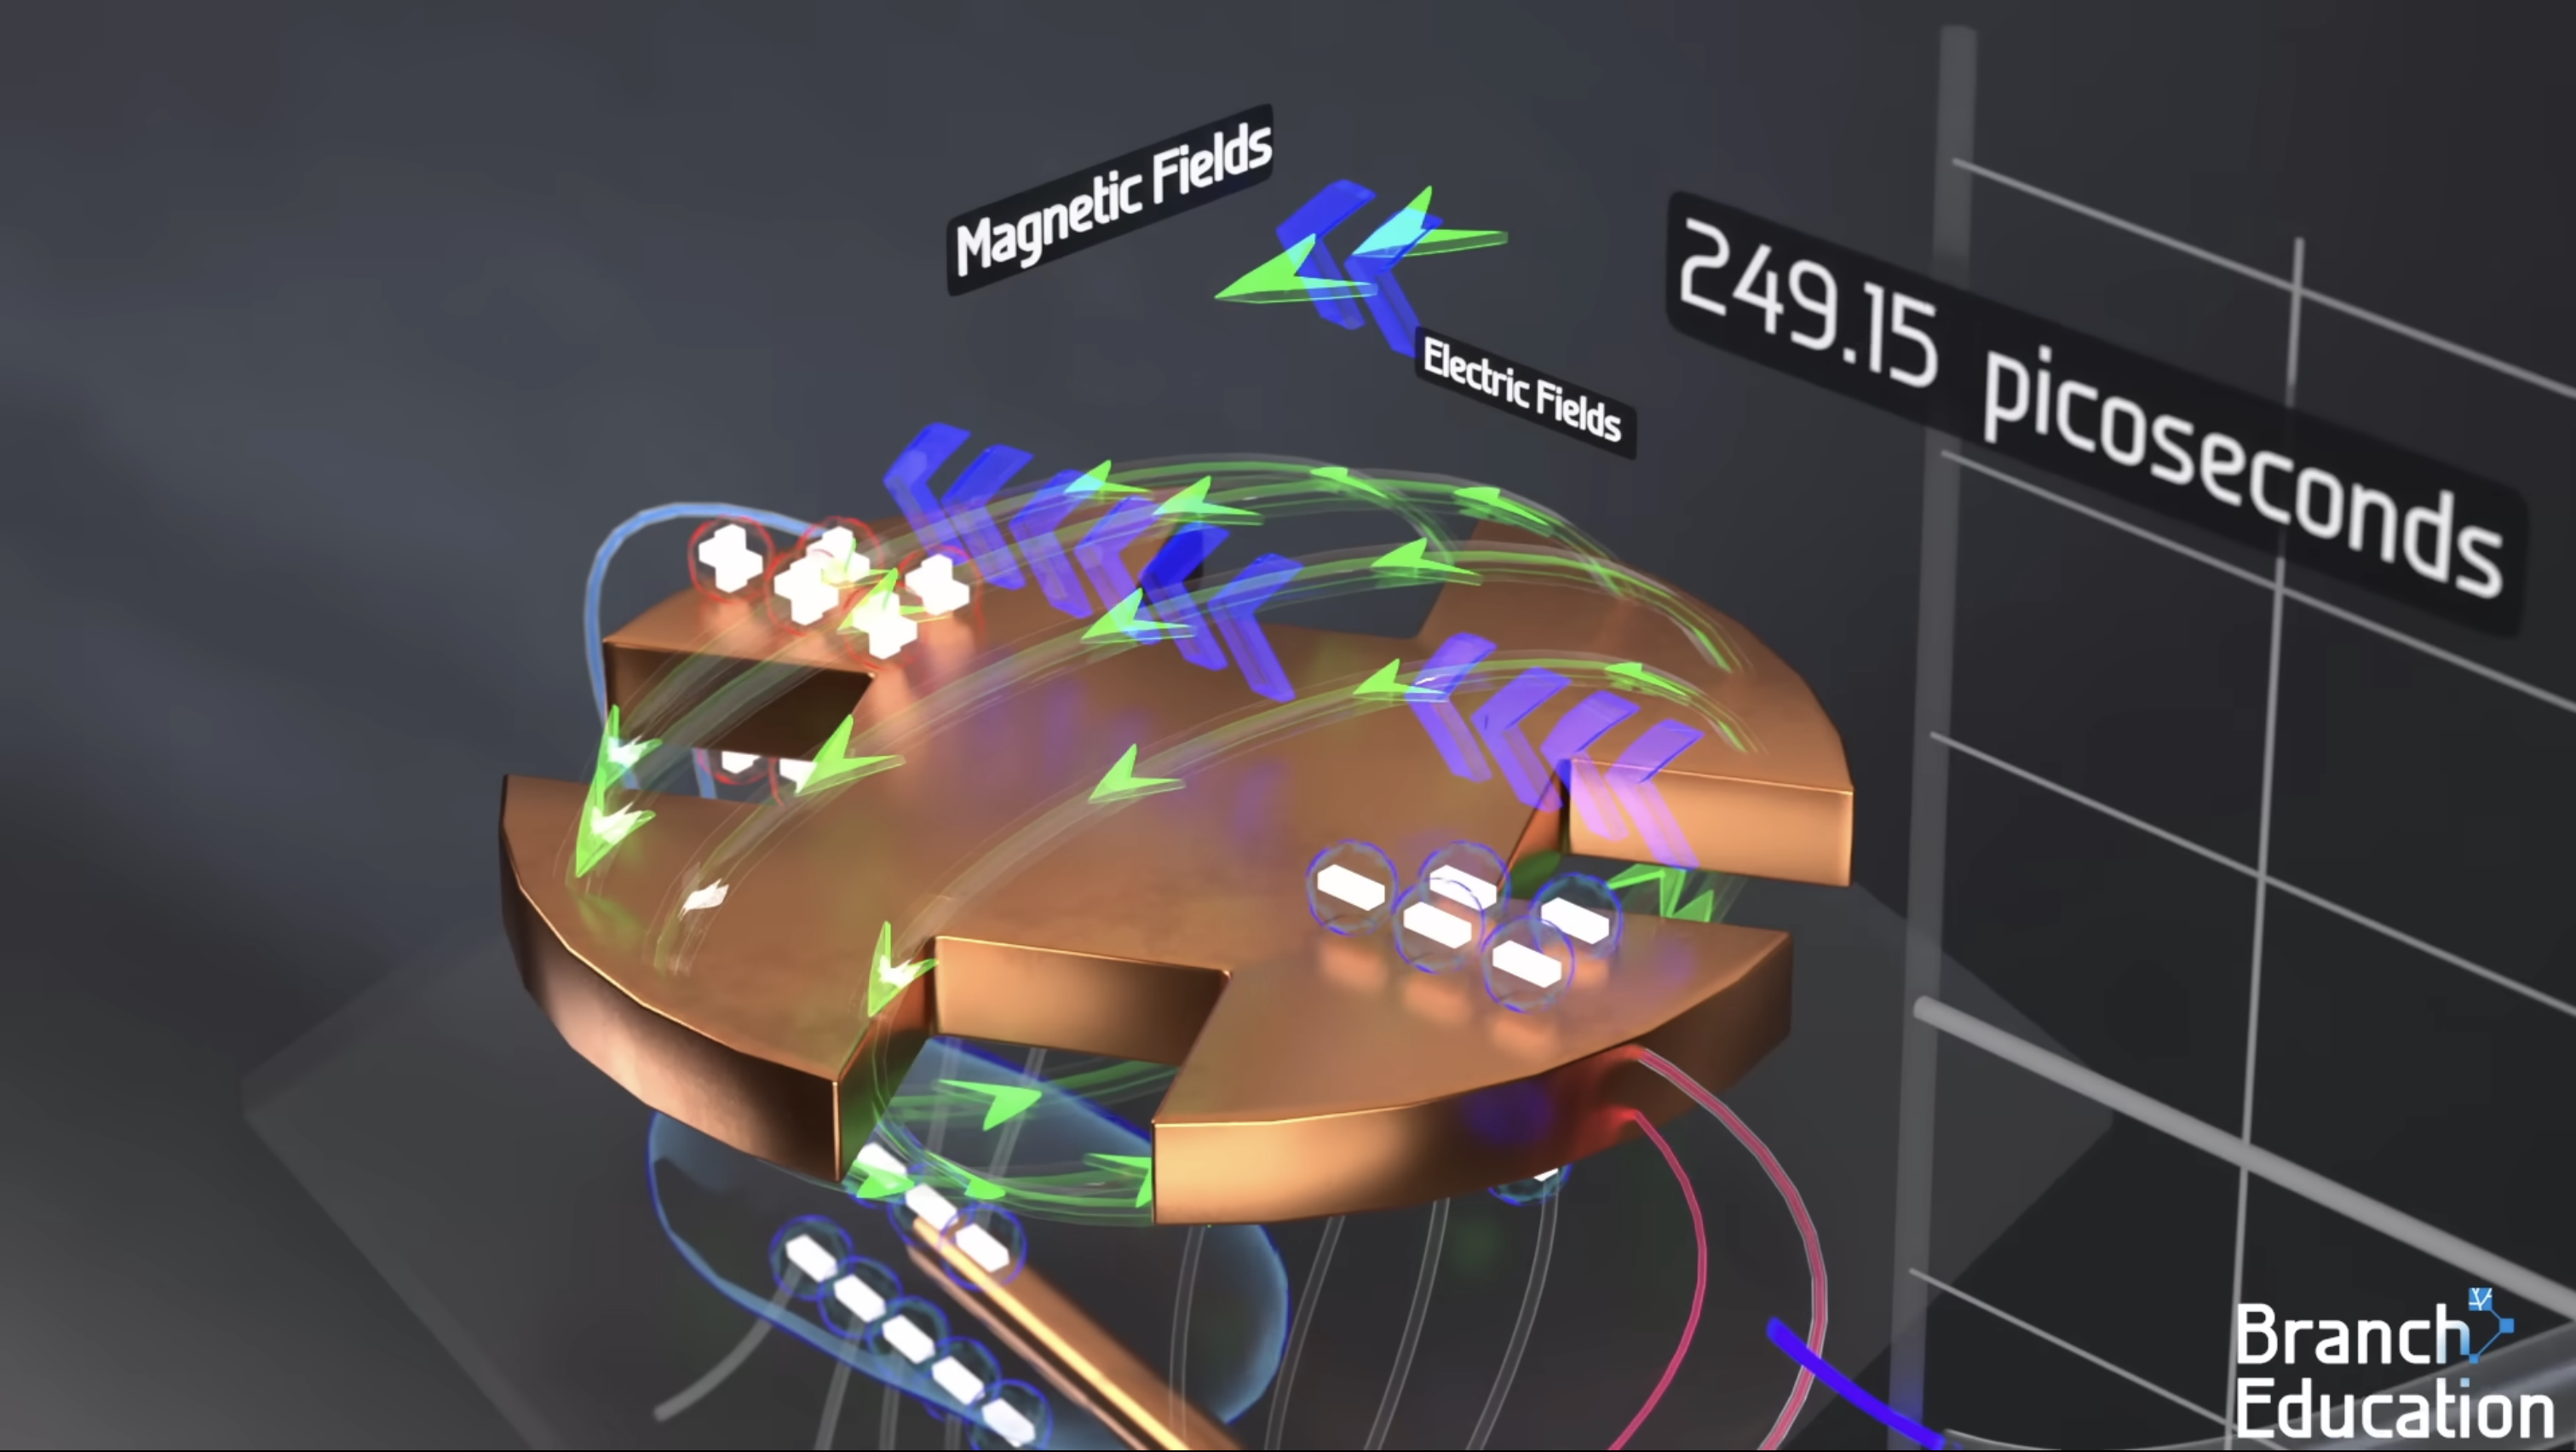
\includegraphics[width=0.8\linewidth]{./res/img/antenna_em_field.png}
  \caption{Campo elettromagnetico in un'Aperture Coupled Patch antenna \cite{branch_education_how_2022}.}
  \label{fig:aperture-couple-patch-antenna-em-field}
\end{figure}

41.5 picosecondi dopo, quando la tensione sulla linea di alimentazione diventa positiva, e siamo al picco della sinusoide, la tensione e la corrente sono invertite.
Quindi il campo elettrico e quello magnetico puntano alla direzione opposta.

\subsection{Emissione delle onde elettromagnetiche}
Creando i campi elettromagnetici oscillanti vengono generate onde elettromagnetiche che viaggiano in direzione perpendicolare al campo elettrico e al campo magnetico.
Dato che i due insiemi di campi non sono tutti sullo stesso piano, ma sono curvati, l'onda elettromagnetica che si propaga viaggia verso l'esterno in una forma di guscio che si espande.

L'intensità di questi campi è legata direttamente alla tensione che è stata originariamente mandata alla linea di alimentaizone alla base dell'antenna.
Questo significa che se vogliamo rendere questi campi elettromagnetici più intensi basta aumentare la tensione inviata alla linea di alimentazione.

Per ricevere il segnale basta commutare il microchip dell'antenna, chiamato modulo front-end, che si vede in figura \ref{fig:aperture-couple-patch-antenna} da modalità trasmettitore a modalità ricevitore.

Quando un'onda elettromagnetica dal satellite è diretta verso l'antenna, i campi elettromagnetici del segnale in arrivo influenzano gli elettroni nel patch di rame, generando un flusso di elettroni.

Questo segnale ad alta frequenza ricevuto è inviato alla feedline, dove c'è il modulo di front-end che amplifica il segnale.
Quindi, queste antenne possono essere usate sia per trasmettere che per ricevere onde elettromagnetiche, ma non allo stesso tempo \cite{branch_education_how_2022}.

\subsection{Beamforming: come formare un fascio di onde elettromagnetiche}
Le tecnica di combinare la potenza delle 1280 antenne in un array esagonale è chiamato beamforming.

Come prima cerchiamo di semplificare il concetto vedendo cosa succede per due antenne affiancate.
Come menzionato prima, un'antenna genera un'onda elettromagnetica che si propaga all'esterno a forma di guscio che si espande.
In ogni singolo punto dello spazio c'è solo un vettore di campo elettrico con un'intensità e una direzione, quindi i vettori di campo elettrico delle due antenne si combinano assieme in tutti i punti nello spazio.
In alcune aree, i campi elettrici delle antenne puntano nella stessa direzione con picchi sovrapposti, e quindi per interferenza costruttiva si sommano.
In altri punti invece sono opposti, con un picco e un'avvallamento, e quindi si cancellano per interferenza distruttiva.

\begin{figure}[htbp]
  \centering
  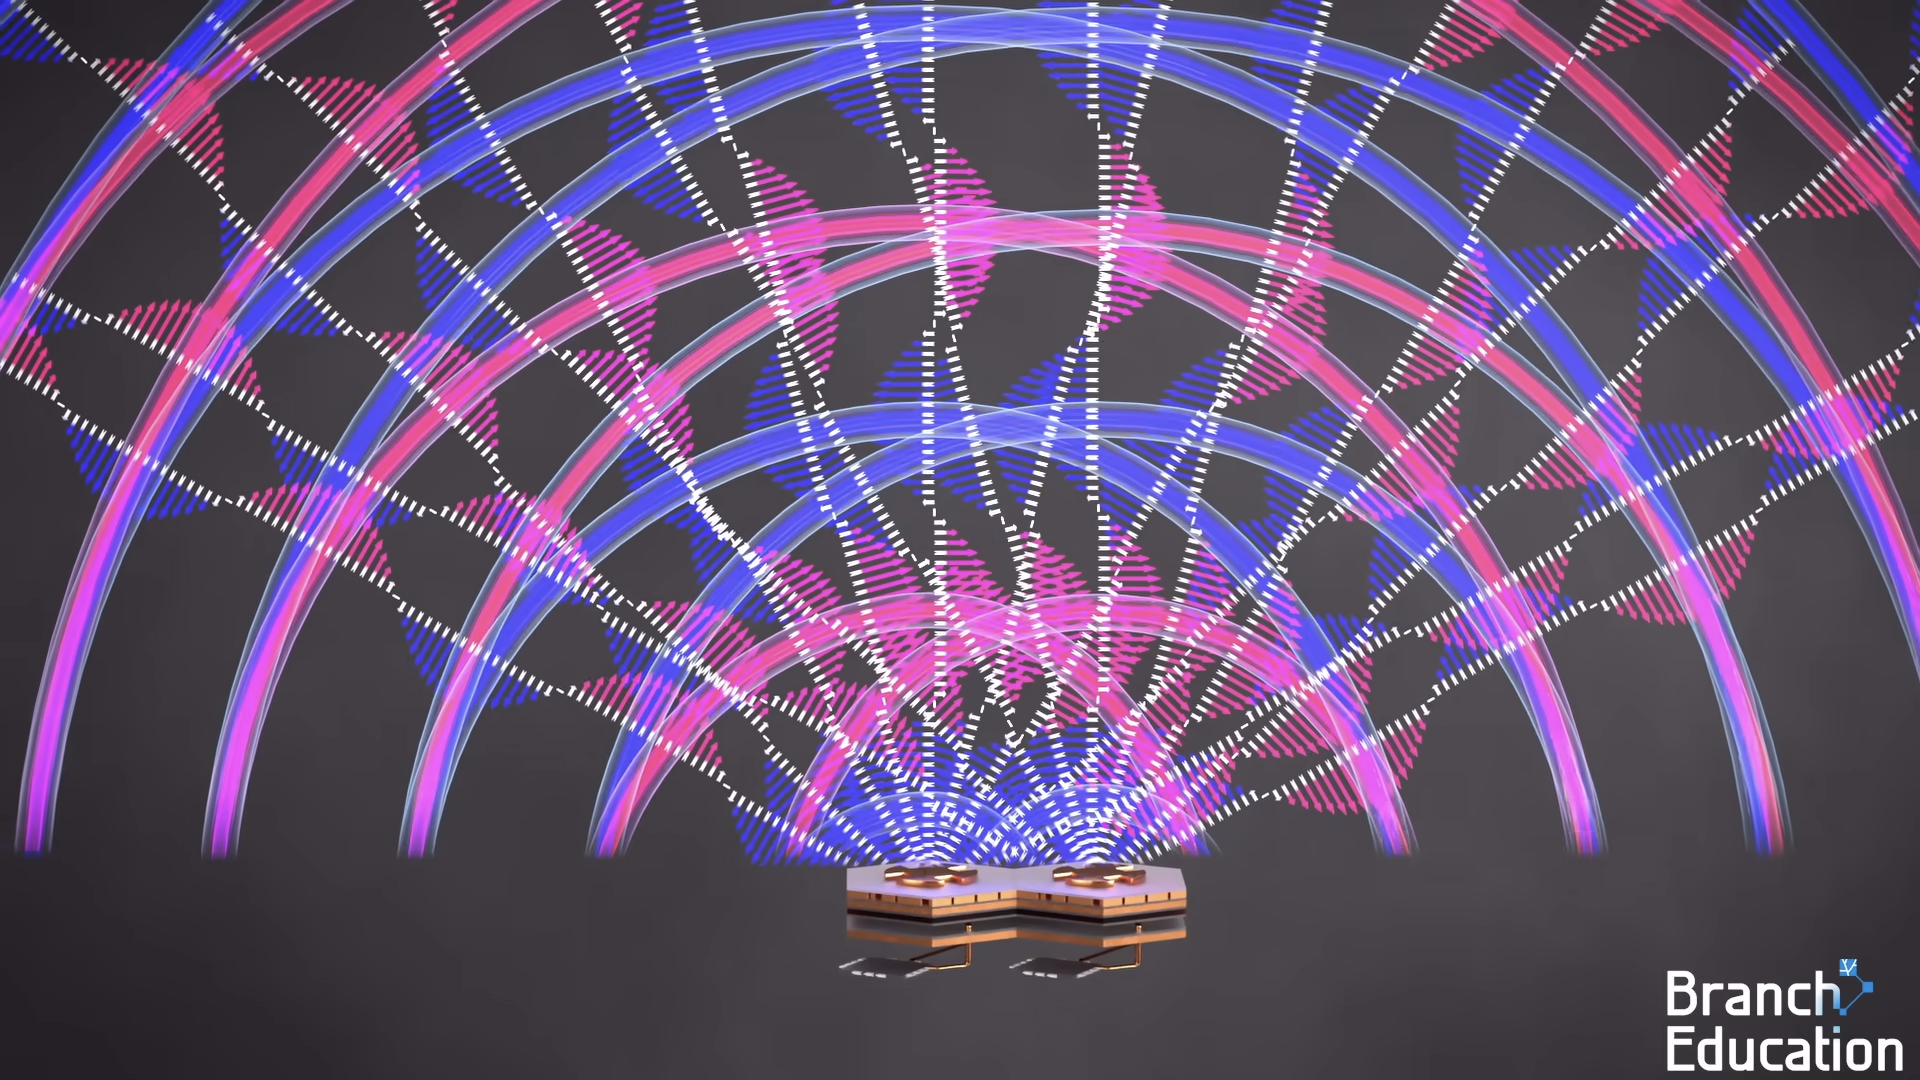
\includegraphics[width=0.8\linewidth]{./res/img/antenna_interference.png}
  \caption{Creazione di interferenze in un array di antenne Aperture Coupled Patch \cite{branch_education_how_2022}.}
  \label{fig:aperture-couple-patch-antenna-interference}
\end{figure}

Quando combiniamo ancora più antenne la zona di interferenza costruttiva diventa ancora più focalizzata rispetto a una singola antenna, in quello che viene chiamato fronte del fascio.
Così, combinando 1280 antenne, possiamo formare un fascio con un'intensità e una direzionalità tali da raggiungere lo spazio \cite{branch_education_how_2022}.

\subsection{Beam Steering: direzionare un fascio di onde elettromagnetiche}
Come menzionato precedentemente dobbiamo direzionare le onde elettromagnetiche per puntare al satellite starlink che viaggia in orbita \ac{LEO} a 27000 km/h.
Usare i motori dell'antenna non è abbastanza preciso e creerebbe stress inutile sui motori.
La soluzione è quindi di usare quello che viene chiamato Phased Array Beam Steering.

Torniamo ancora una volta all'esempio delle due antenne.
Prima stavamo inviando lo stesso segnale alle due antenne, e quindi queste erano in fase l'una con l'altra.
Per fare beam steering invece si invia il segnale alle antenne con una differenza di fase per poterlo angolare.
Come risultato i tempi dei picchi e delle valli emesse da un'antenna sono differenti dalle altre.
In questo modo le posizioni delle interferenze costruttive sono angolati verso una certa direzione, con interferenze distruttive da tutte le altre parti.
Quindi, cambiando continuamente la fase del segnale inviato all'antenna possiamo creare una zona di sweeping di interferenza costruttiva.

Per sapere l'angolo esatto a cui il fascio di onde deve essere indirizzato si usano le coordinate GPS dell'antenna tramite il suo chip GPS, insieme alle posizioni orbitali del satellite Starlink che è conosciuto nel software dell'antenna.
Il software calcola l'angolo e lo shift di fase richiesto per ciascuna delle antenne.
I risultati dei calcoli del phase shift sono successivamente inviati ai 20 chip più grandi chiamati beamformers, e ciascun beamformer coordina 32 chip più piccoli chiamati moduli di front end, ciascuno dei quali controlla 2 antenne.
Ogni pochi microsecondi questi calcoli sono aggiornati e distribuiti in tutto il PCB dell'antenna in modo da orientare perfettamente il segnale verso il satellite.
Come risultato, il raggio può essere orientato ovunque in un campo visivo di 100 gradi \cite{branch_education_how_2022}.